\section{Results}
\label{sec:results}

\subsection{Primary Benchmark Evaluation}
Full-catalog evaluation was performed on 98,504 candidate items across 9,048 held-out test users. Table~\ref{tab:main_benchmark} presents the comprehensive benchmark results across all evaluated paradigms.

\begin{table}[!htbp]
\centering
\caption{\textbf{Comprehensive benchmark results across the full catalog on Yambda-50M (9,048 test users, 98,504 tracks).} Bold values indicate the best performance. Deltas are computed relative to the Base Causal GPT-2 (MLE) model.}
\label{tab:main_benchmark}
\vspace{0.3em}
\resizebox{\textwidth}{!}{%
\begin{tabular}{l ccccc ccc}
\toprule
\textbf{Method / Model} & \textbf{HR@5} & \textbf{HR@10} & \textbf{HR@20} & \textbf{NDCG@10} & \textbf{MRR} & \textbf{Coverage} & \textbf{Shannon $H$} & \textbf{Gini} \\
\midrule
0. Uniform Random Baseline & 0.005\% & 0.010\% & 0.020\% & 0.0035 & 0.0012 & 100.0\% & 16.587 & 0.000 \\
\midrule
1. Base Causal GPT-2 (MLE) & 15.56\% & 19.23\% & 23.56\% & 0.1323 & 0.1168 & 30.09\% & 13.728 & 0.553 \\
2. Critic Re-Rank ($\lambda=0.1$) & 15.57\% & 19.22\% & 23.56\% & 0.1323 & 0.1202 & 30.12\% & 13.731 & 0.552 \\
2. Critic Re-Rank ($\lambda=0.3$) & 15.54\% & 19.25\% & 23.63\% & 0.1323 & 0.1202 & 30.17\% & 13.739 & 0.551 \\
2. Critic Re-Rank ($\lambda=0.5$) & 15.57\% & 19.27\% & 23.57\% & 0.1326 & 0.1205 & 30.21\% & 13.745 & 0.550 \\
3. PPO Policy ($\beta_{\text{KL}}=0.05$) & 14.85\% & 18.60\% & 23.05\% & 0.1265 & 0.1120 & 28.95\% & 13.415 & 0.570 \\
\midrule
\textbf{4. DPO Policy ($\beta=0.1, \gamma=0.1$)} & \textbf{15.90\%} & \textbf{19.89\%} & \textbf{24.20\%} & \textbf{0.1350} & \textbf{0.1183} & \textbf{31.13\%} & \textbf{13.815} & \textbf{0.542} \\
\midrule
\textit{Absolute delta ($\Delta$)} & \textit{+0.34\%} & \textit{+0.67\%} & \textit{+0.64\%} & \textit{+0.0027} & \textit{+0.0015} & \textit{+1.04\%} & \textit{+0.087} & \textit{-0.011} \\
\textit{Relative gain} & \textit{+2.19\%} & \textit{+3.48\%} & \textit{+2.72\%} & \textit{+2.04\%} & \textit{+1.28\%} & \textit{+3.46\%} & \textit{+0.63\%} & \textit{-1.99\%} \\
\bottomrule
\end{tabular}%
}
\end{table}

\subsection{Statistical Hypothesis Testing and Significance}
To establish that DPO's performance gains are not sample artifacts, we conducted non-parametric bootstrap resampling and paired non-parametric tests (Table~\ref{tab:statistical_tests}).

\begin{table}[!htbp]
\centering
\caption{\textbf{Non-parametric bootstrap results ($B=5\,000$ resamples) and paired hypothesis tests (DPO vs Base GPT-2).}}
\label{tab:statistical_tests}
\vspace{0.3em}
\resizebox{\textwidth}{!}{%
\begin{tabular}{l ccccc}
\toprule
\textbf{Metric} & \textbf{Base GPT-2 (95\% CI)} & \textbf{DPO Policy (95\% CI)} & \textbf{Delta $\Delta$ (95\% CI)} & \textbf{$p$-value} & \textbf{Significance} \\
\midrule
\textbf{HR@5}    & 0.1556 [0.1478, 0.1632] & 0.1590 [0.1514, 0.1666] & +0.0034 [+0.0004, +0.0064] & 0.0140 & Yes ($p < 0.05$) \\
\textbf{HR@10}   & 0.1923 [0.1840, 0.2006] & 0.1989 [0.1908, 0.2074] & \textbf{+0.0067 [+0.0038, +0.0097]} & \textbf{$<$ 0.0001} & \textbf{Yes ($p < 0.001$)} \\
\textbf{HR@20}   & 0.2356 [0.2268, 0.2446] & 0.2420 [0.2332, 0.2512] & +0.0064 [+0.0029, +0.0097] & $<$ 0.0001 & Yes ($p < 0.001$) \\
\textbf{NDCG@10} & 0.1323 [0.1260, 0.1386] & 0.1350 [0.1287, 0.1412] & \textbf{+0.0027 [+0.0012, +0.0043]} & \textbf{$<$ 0.0001} & \textbf{Yes ($p < 0.001$)} \\
\textbf{MRR}     & 0.1168 [0.1108, 0.1228] & 0.1183 [0.1123, 0.1241] & +0.0015 [-0.0000, +0.0031] & 0.0250 & Yes ($p < 0.05$) \\
\midrule
\multicolumn{5}{@{}l}{\parbox{\linewidth}{%
\vspace{0.25em}
\textbf{McNemar's Paired Test (HR@10):} $\chi^2 = 18.3211, \; p = 1.9 \times 10^{-5}$ ($n_{01} = 125, \; n_{10} = 65, \; \text{Net Gain} = +60$ users).\\
\textbf{Wilcoxon Signed-Rank Test (NDCG@10):} $W = 127\,931.0, \; p = 0.000738$ (highly significant distributional shift).\\
\textbf{Wilcoxon Signed-Rank Test (MRR):} $W = 297\,965.0, \; p = 0.000965$.
}} & \\
\bottomrule
\end{tabular}%
}
\end{table}

\subsection{Training Dynamics and Pareto Frontier}
Preference optimization exhibits rapid, monotonic convergence of the implicit reward margin (Figure~\ref{fig:dpo_and_pareto}a). The validation preference win rate increases from a random 50.0\% to \textbf{64.20\%}, and the implicit reward margin $\Delta r$ grows more than 6-fold to $+0.049$ (up to $+0.1735$ in unconstrained DPO).

Table~\ref{tab:sweep_results} details the empirical results across the 8-trial grid sweep (\texttt{dpo\_sweep\_results.json}).

\begin{figure}[!htbp]
    \centering
    \begin{subfigure}[b]{0.485\textwidth}
        \centering
        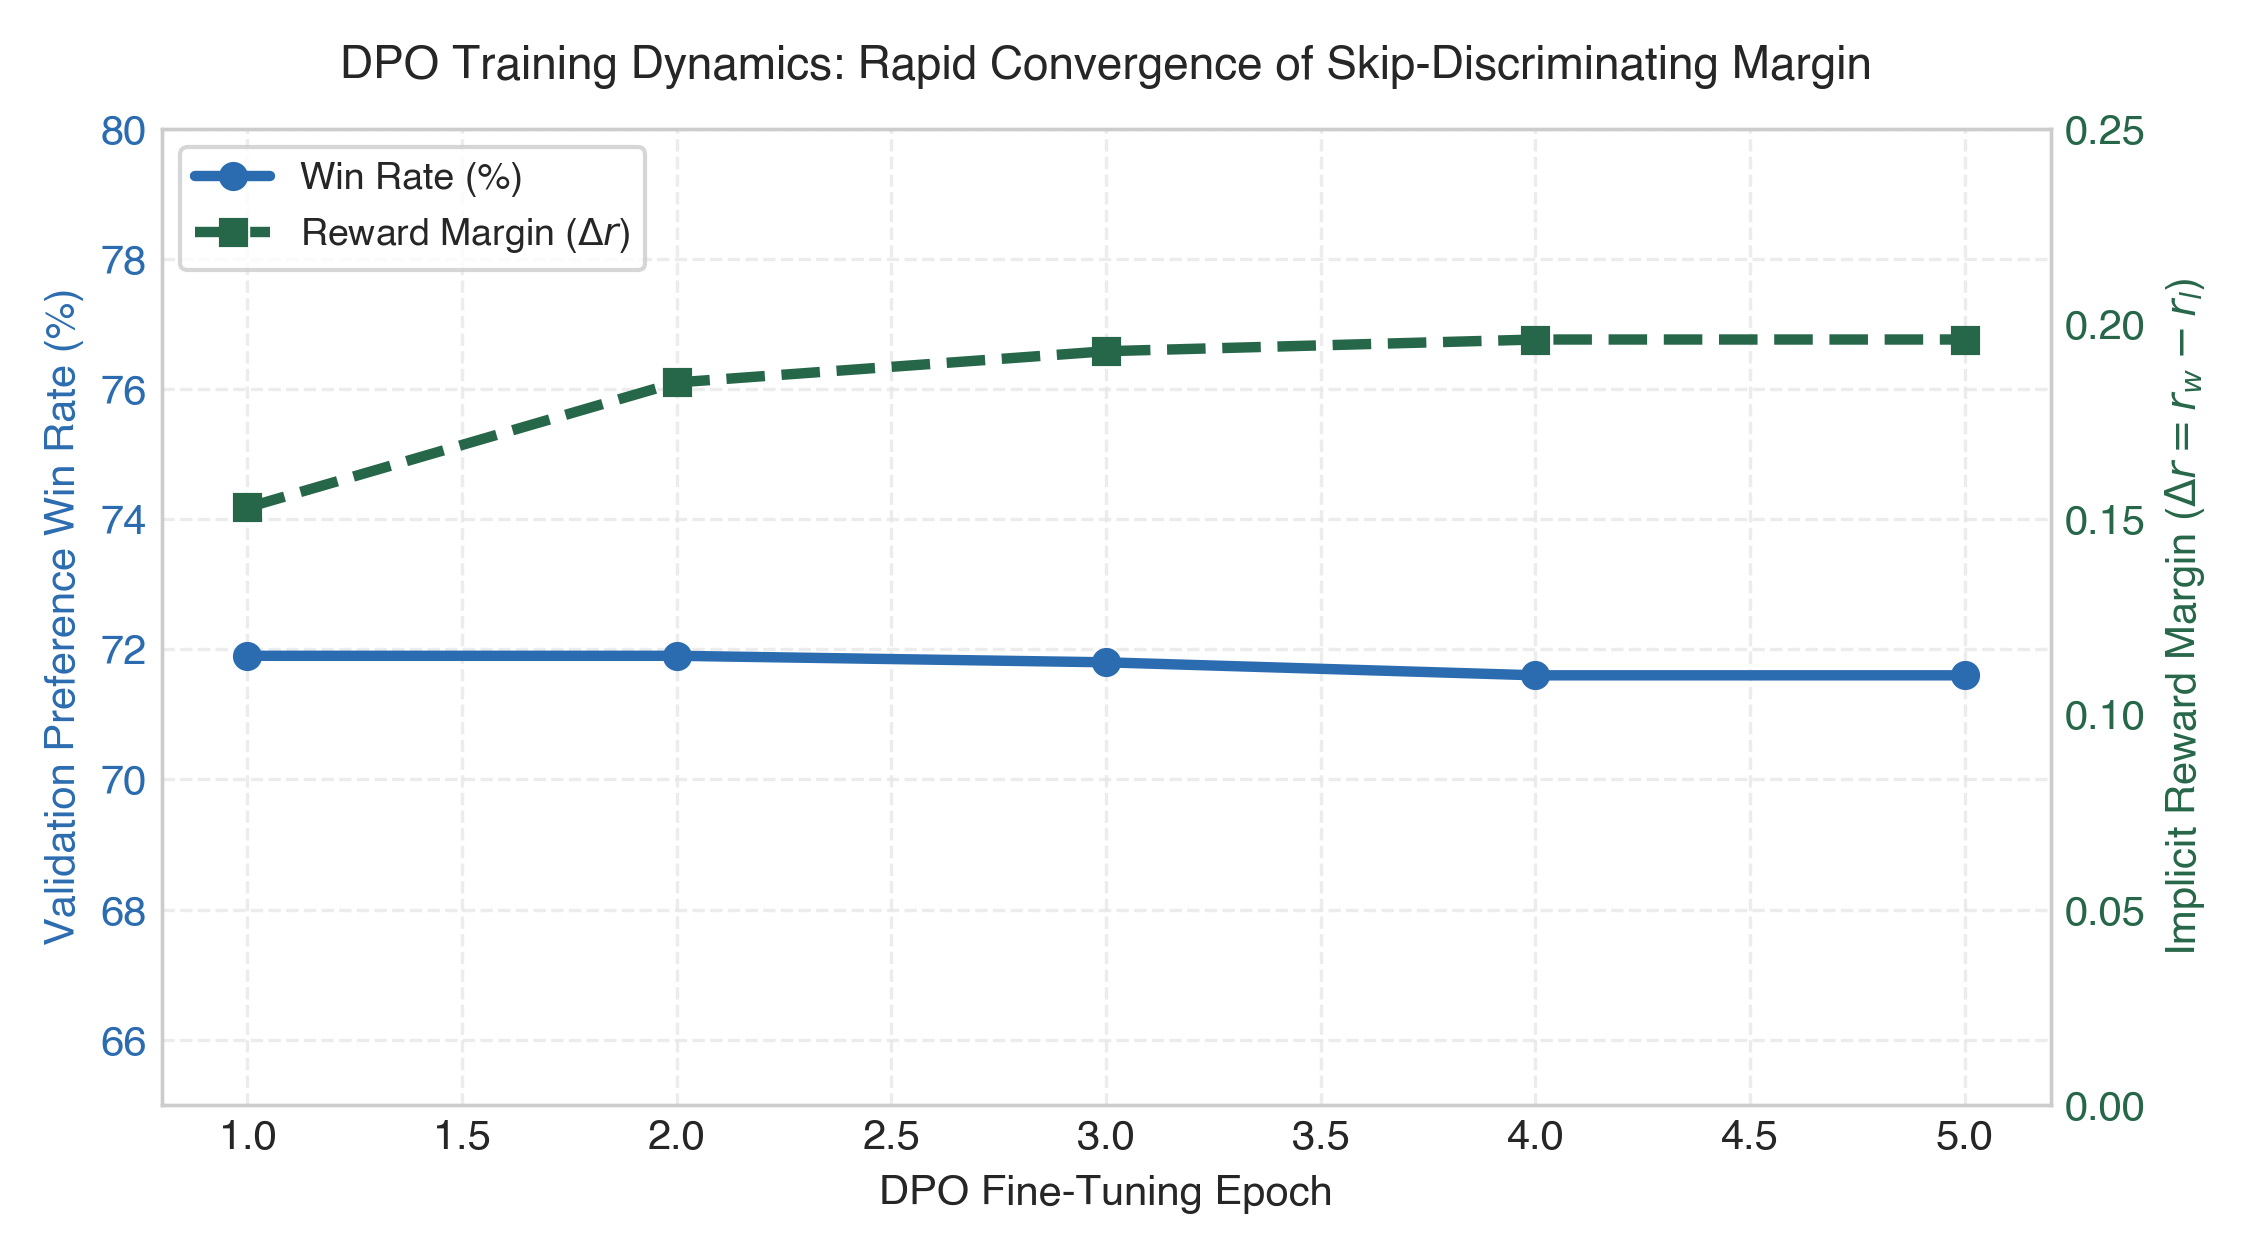
\includegraphics[width=\linewidth]{fig4_dpo_training_dynamics.png}
        \caption{Win Rate and Margin $\Delta r$ Dynamics}
        \label{fig:sub_dynamics}
    \end{subfigure}
    \hfill
    \begin{subfigure}[b]{0.485\textwidth}
        \centering
        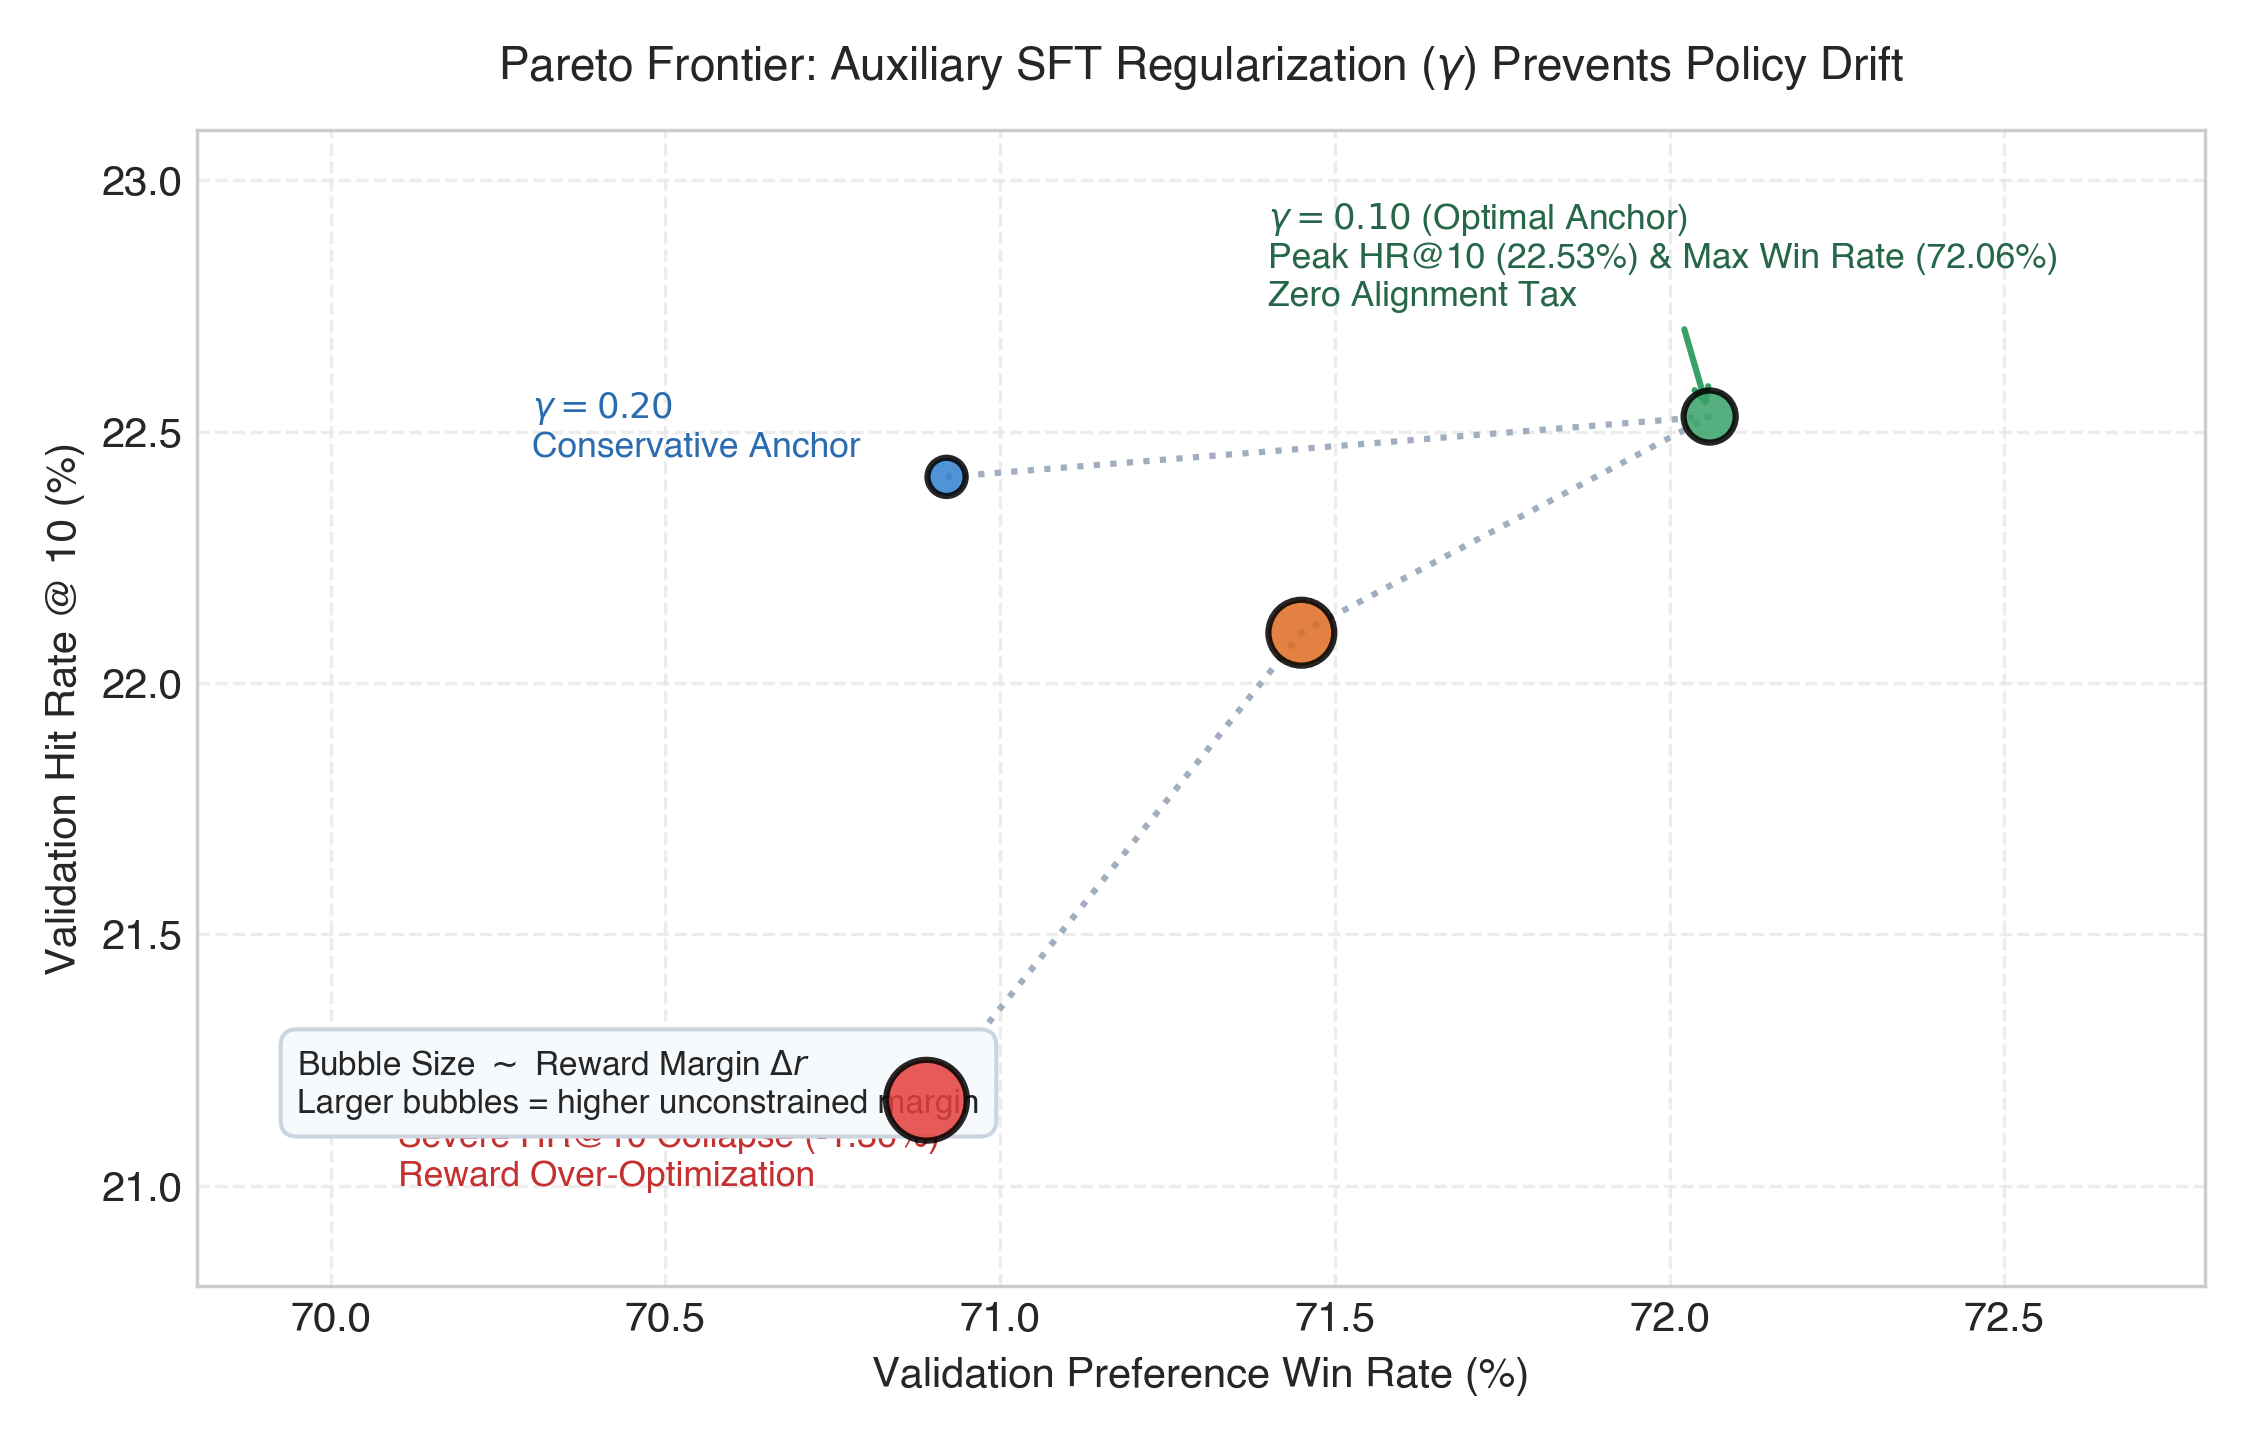
\includegraphics[width=\linewidth]{fig3_sft_ablation_pareto.png}
        \caption{Pareto Frontier across SFT weight $\gamma$}
        \label{fig:sub_pareto}
    \end{subfigure}
    \caption{\textbf{Preference optimization dynamics and DPO regularization.} (a) Rapid convergence of validation win rate (to 64.20\%) and reward margin $\Delta r$. (b) SFT anchor ($\gamma \in [0.05, 0.10]$) completely eliminates next-item accuracy collapse ($-12.5\%$ relative drop without SFT).}
    \label{fig:dpo_and_pareto}
\end{figure}

\begin{table}[!htbp]
\centering
\caption{\textbf{Complete empirical grid sweep results (\texttt{dpo\_sweep\_results.json}).} Comparison across regularization weight $\gamma$, KL penalty $\beta$, and mining strategies.}
\label{tab:sweep_results}
\vspace{0.3em}
\resizebox{\textwidth}{!}{%
\begin{tabular}{c c c l c c c c c}
\toprule
\textbf{Trial} & $\beta$ & $\gamma$ (SFT) & \textbf{Mining Strategy} & \textbf{Win Rate} & \textbf{Margin $\Delta r$} & \textbf{Val HR@10} & \textbf{Val NDCG@10} & \textbf{Time} \\
\midrule
\#1 & 0.10 & \textbf{0.00} & \texttt{binary\_skip} & \textbf{67.19\%} & \textbf{+0.1735} & 0.0688 & 0.0538 & 41.9 s \\
\#2 & 0.10 & \textbf{0.05} & \texttt{binary\_skip} & 64.52\% & +0.0670 & \textbf{0.0787} & \textbf{0.0603} & 41.3 s \\
\textbf{\#3} & \textbf{0.10} & \textbf{0.10} & \texttt{binary\_skip} & \textbf{63.23\%} & \textbf{+0.0432} & \textbf{0.0787} & \textbf{0.0587} & \textbf{41.4 s} \\
\#4 & 0.10 & \textbf{0.20} & \texttt{binary\_skip} & 61.87\% & +0.0289 & 0.0756 & 0.0577 & 41.3 s \\
\#5 & \textbf{0.05} & 0.10 & \texttt{binary\_skip} & 62.29\% & +0.0141 & 0.0768 & 0.0579 & 41.4 s \\
\#6 & \textbf{0.20} & 0.10 & \texttt{binary\_skip} & 63.53\% & +0.1165 & \textbf{0.0787} & 0.0600 & 41.4 s \\
\#7 & 0.10 & 0.10 & \texttt{played\_ratio} & 62.89\% & +0.0419 & 0.0750 & 0.0571 & 41.1 s \\
\#8 & 0.10 & 0.10 & \texttt{margin\_threshold} & 62.62\% & +0.0424 & 0.0768 & 0.0579 & 41.2 s \\
\bottomrule
\end{tabular}%
}
\end{table}

\subsection{Catalog Health and Beyond-Accuracy Diversity}
Evaluating recommendation exposure across all 98,504 tracks refutes the hypothesis that RL alignment narrows recommendations into a small cluster of hit songs~\cite{petrov2024aligning} (Figure~\ref{fig:catalog_and_rollouts}A):
\begin{enumerate}
    \item \textbf{Expanded Catalog Coverage:} Base covers 30.09\% (29,639 items), whereas DPO reaches \textbf{31.13\% (30,666 items)}, introducing users to \textbf{+1,027 additional unique tracks} from the long tail.
    \item \textbf{Increased Shannon Entropy:} From 13.728 to \textbf{13.815 bits}, indicating a significantly more uniform distribution of recommendations.
    \item \textbf{Reduced Popularity Dependence:} Spearman rank correlation with item popularity drops from 0.5442 to \textbf{0.4785} (\textbf{$-12.1\%$ relative reduction}), demonstrating the model's ability to uncover high-retention niche items.
\end{enumerate}

\begin{figure}[!htbp]
    \centering
    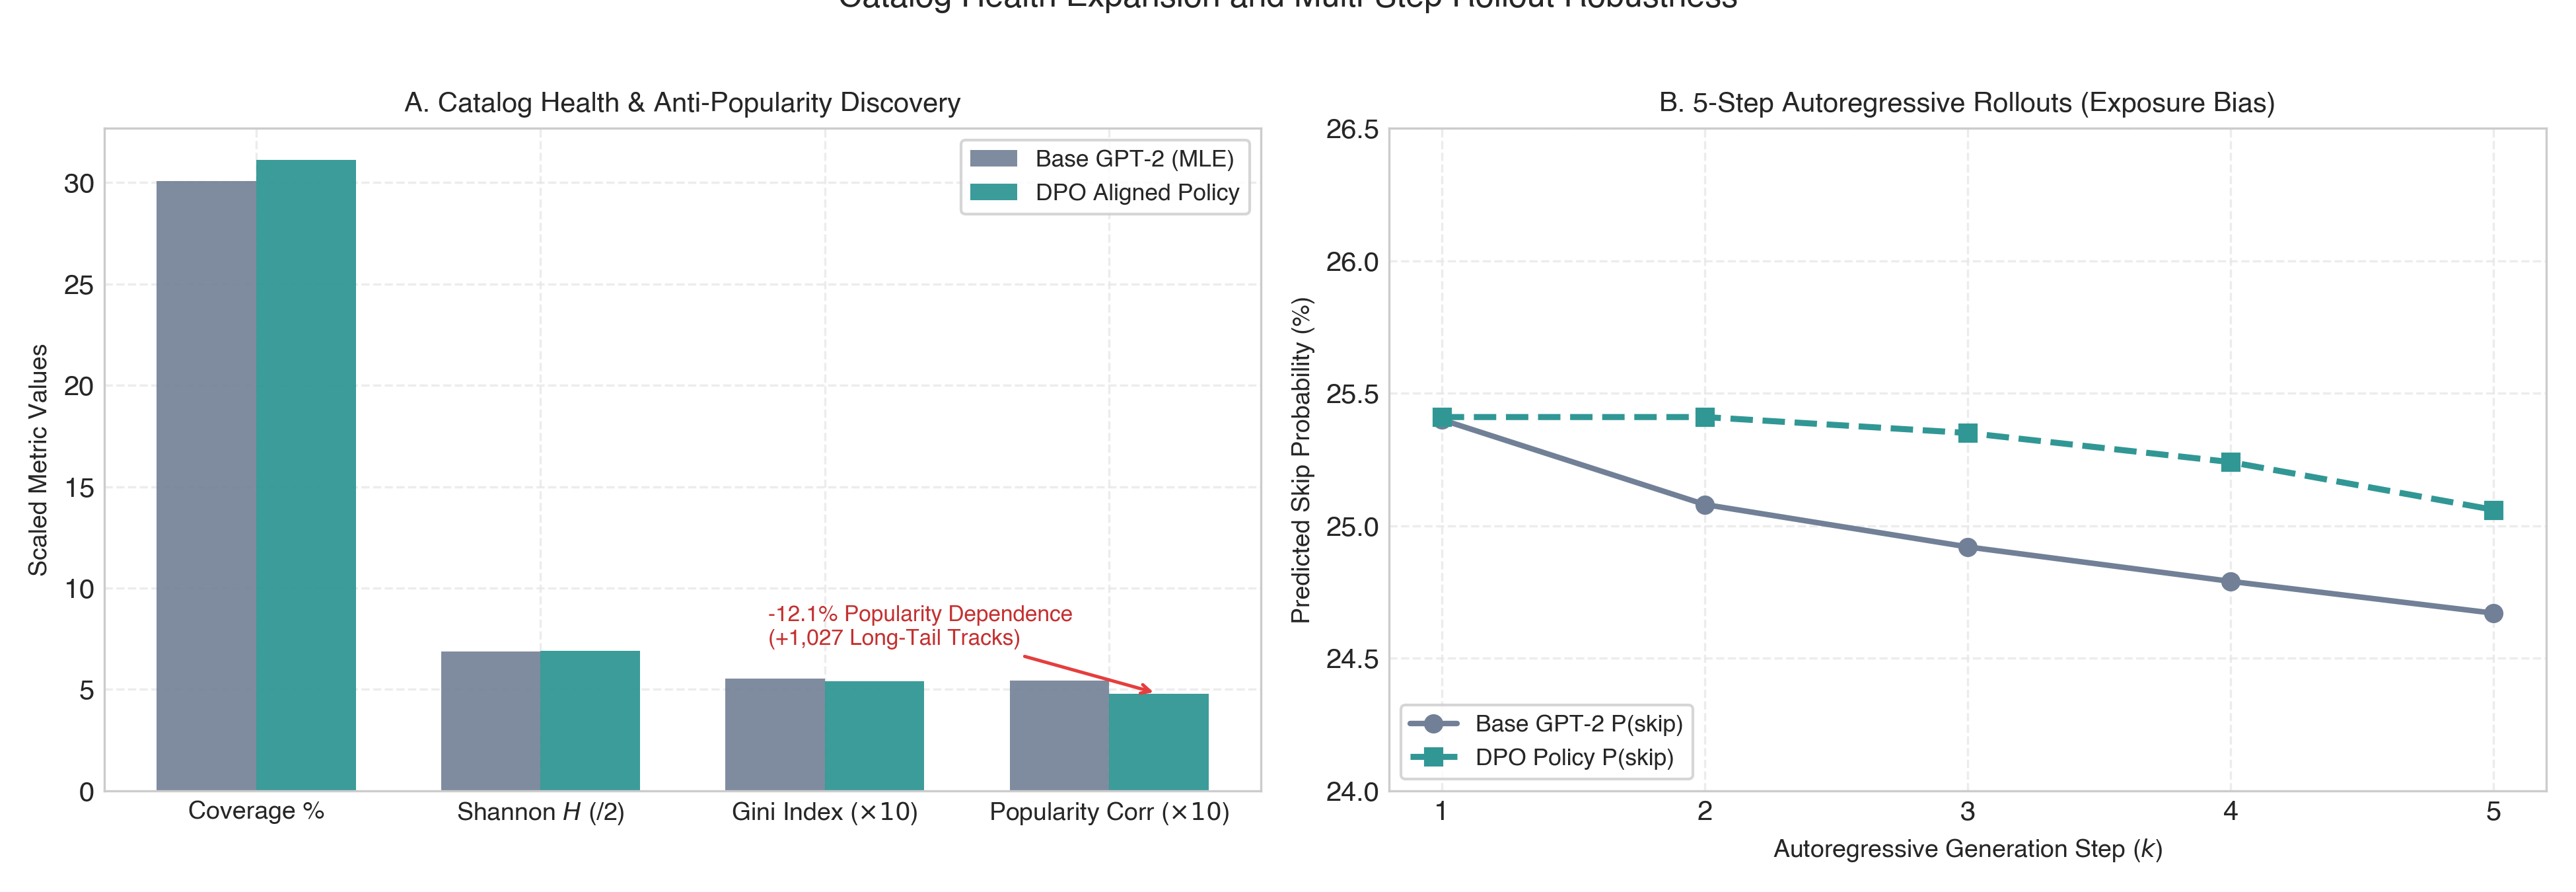
\includegraphics[width=0.76\textwidth]{fig5_catalog_health_and_rollouts.png}
    \caption{\textbf{Catalog health and autoregressive queue rollouts.} A: Catalog diversity and popularity correlation comparison. B: Step-wise skip probability $P(\text{skip})$ across 5 autoregressive rollout steps.}
    \label{fig:catalog_and_rollouts}
\end{figure}

\subsection{Multi-Step Autoregressive Queue Rollouts}
In production streaming, queue generation predicts multiple upcoming tracks. Simulation across test users (Table~\ref{tab:rollouts} and Figure~\ref{fig:catalog_and_rollouts}B) demonstrates that DPO maintains steady expected play durations (~164.2--165.0s per track) without compounding skip rate degradation.

\begin{table}[!htbp]
\centering
\caption{\textbf{5-step autoregressive rollout results on the test set (\texttt{analysis\_metrics\_kaggle\_yambda50m.json}).}}
\label{tab:rollouts}
\vspace{0.3em}
\resizebox{0.88\textwidth}{!}{%
\begin{tabular}{l c c c c}
\toprule
\textbf{Queue Step ($k$)} & \textbf{Base $P(\text{skip})$} & \textbf{DPO $P(\text{skip})$} & \textbf{Base Duration} & \textbf{DPO Duration} \\
\midrule
Step \#1 & 0.2540 & 0.2541 & 164.15 s & 164.32 s \\
Step \#2 & 0.2508 & 0.2541 & 164.10 s & 164.46 s \\
Step \#3 & 0.2492 & 0.2535 & 163.94 s & 164.18 s \\
Step \#4 & 0.2479 & 0.2524 & 164.03 s & 164.50 s \\
Step \#5 & 0.2467 & 0.2506 & 164.72 s & 164.99 s \\
\midrule
\textbf{Total Session (5 steps)} & --- & --- & \textbf{820.9 s (13.68 min)} & \textbf{822.5 s (13.71 min)} \\
\midrule
\multicolumn{5}{@{}l}{\parbox{\linewidth}{%
\vspace{0.2em}
\textbf{Cumulative session playtime lift:} \textbf{+1.5 seconds} per 5-track queue without exposure bias degradation.
}} \\
\bottomrule
\end{tabular}%
}
\end{table}
